\documentclass[t]{beamer}

\subtitle{Section 2.10: The First Isomorphism Theorem}

\input{../../_tools/setup}

\begin{document} 
	\startdoc
	
	\topics{
		\item Factor Groups
		\item Commutator Subgroups
	}{
		\item Kernels
		\item The first isomorphism theorem
	}

\slide{
	\begin{defn}
		Let $\alpha:G\to H$ be a group homomorphism.  The \emph{image of $\alpha$} is the set
			\[\im\alpha=\alpha(G)=\{\alpha(g)\ |\ g\in G\}.\]
			
		The \emph{kernel of $\alpha$} is the set
			\[\ker\alpha=\{k\in G\ |\ \alpha(k)=e_H\}.\]
	\end{defn}
	\begin{exercise}
		Let $\alpha:\Z\to \C^*$ be defined by $\alpha(n)=i^n$ where $i=\sqrt{-1}$.
		
		Compute $\ker(\alpha)$.  
	\end{exercise}
}


\slide{
	\begin{thm}{Almost 2.10.1}
		If $\alpha:G\to H$ is a group homomorphism, then $\ker\alpha$ is a subgroup of $G$.
	\end{thm}
	\begin{exercise}
		Let $\alpha:\Z\to \C^*$ be defined by $\alpha(n)=i^n$ where $i=\sqrt{-1}$.
		
		What are the cosets of $\ker(\alpha)$?
	\end{exercise}
}
%\slide{
%	\begin{block}{\textbf{Observation.}}
%		If $a\ker(\phi)=b\ker(\phi)$, then $\phi(a)=\phi(b)$!  We'll come back to this soon.
%	\end{block}
%}
\slide{
	\begin{thm}{2.10.1}
		Let $\alpha:G\to H$ be a group homomorphism.  Then
		\enumarabic{\item $\alpha(G)$ is a subgroup of $H$. \item $\ker(\phi)$ is a \textbf{normal} subgroup of $G$}
	\end{thm}
	\begin{proof} We will show $\ker(\phi)\lhd G$.
		\vskip 1.75in
	\end{proof}
}
\slide{
	\begin{exercise}
		\enumalph{\item Prove $SL_2(\R)\lhd GL_2(\R)$.\vskip 1in \item Prove $A_n\lhd S_n$.\vskip 1in \mbox{}}
	\end{exercise}
}
\slide{\begin{question}
		\enumarabic{\item If $\phi$ is surjective, then $\phi(G)$ is the largest it can be?\vskip .75in \item If $\phi$ is the trivial homomorphism, then $\ker(\phi)$ is the largest it can be?\vskip .75in\item If $\ker(\phi)$ is as small as it can be then is $\phi$ surjective?\vskip .75in\mbox{}}
\end{question}}
\slide{
	\begin{thm}{2.10.3}
		Let $\alpha:G\to H$ be a group homomorphism.  Then $\alpha$ is injective if and only if $\ker(\alpha)=\{e_G\}$.
	\end{thm}
}

\slide{
	\begin{statementblock}{The First Isomorphism Theorem (2.10.4)}
		Let $\alpha: G\to H$ be a group homomorphism then $G/K\cong im(G)=\alpha(G)$.
	\end{statementblock}
}

\slide{
	So here we have a map $\alpha:G\to H$. Let $K=\ker(\alpha)$. 
		\vskip 2em
	Define $\overline{\alpha}: G/K\to im(\alpha)$ given by $\overline{\alpha}(aK)=\alpha(a)$.
		\vskip 2em
	Claim: $\overline{\alpha}$ is an isomorphism.
	
	\begin{nb}
		Since the domain of $\alpha$ is a quotient, we have to first make sure that $\alpha$ is well-defined. **Elements in the domain can be represented in multiple ways.**
	\end{nb}
}

\slide{
	\begin{proof}[Proof ($\overline{\alpha}$ is well-defined and one-to-one).]
		\vskip 2.5in
	\end{proof}
}
\slide{
\begin{proof}[Proof ($\overline{\alpha}$ is onto).]
	\vskip 2.5in
\end{proof}
}
\slide{
\begin{proof}[Proof ($\overline{\alpha}$ is a homomorphism)]
	\vskip 2.5in
\end{proof}
}
\slide{
	\begin{exercise}
		Prove that $\Z/n\Z\cong \Z_n$ for all integers $n\geq 1$.
	\end{exercise}
}
\begin{frame}[fragile]
	\frametitle{\fn}
	\begin{recall}
		If $a+bi\in \C$ for $a,b\in\R$, we can plot this as the point $(a,b)$.
		
		Moreover, any point on unit circle corresponds to the complex number $e^{i\theta}$ where $\theta$ is the angle between the vector defined by the point and the positive $x$-axis:
		
		\begin{center}
			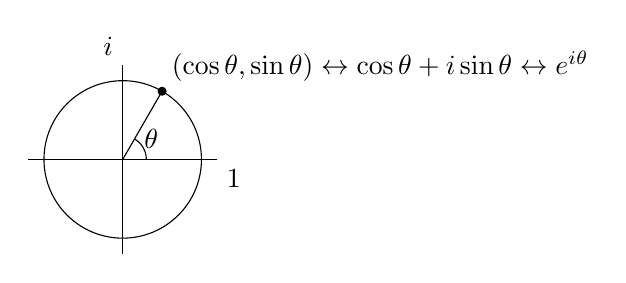
\begin{tikzpicture}
				\draw (0,0) circle (1);
				\filldraw (0,0) -- (60:1) circle (.05) node[anchor=south west] {$(\cos\theta,\sin\theta)\leftrightarrow \cos\theta+i\sin\theta\leftrightarrow e^{i\theta}$};
				\draw (.3,0) arc (0:60:.3) node[anchor=west] {$\theta$};
				\draw (-1.2,0) -- (1.2,0) node[anchor=north west] {$1$};
				\draw (0,-1.2) -- (0,1.2) node[anchor=south east] {$i$};
			\end{tikzpicture}
		\end{center}
		
		
		Claim: The unit circle,$$\C^0 = \{z\in \C:|z|=1\}=\{e^{i\theta} : 0\leq \theta < 2\pi\}=\{e^{i\theta} : \theta\in \R\}$$ is a subgroup of $\C^\times$ (operation is multiplication).
	\end{recall}
\end{frame}
\slide{
	\begin{exercise}
		Prove that $\R/\Z$ (under addition) is isomorphic to $\C^0$ (under multiplication).
	\end{exercise}
}

\slide{
	\begin{statementblock}{Claim}
		If $K_1\lhd G_1$ and $K_2\lhd G_2$, then $K_1\times K_2\lhd G_1\times G_2$ and 
		\[(G_1\times G_2)/(K_1\times K_2)\cong G_1/K_1\times G_2/K_2.\]
	\end{statementblock}
}
\slide{\begin{exercise}
		Let $D_3=\{e,r,r^2,f,fr,fr^2\}$ with $|r|=3$, $|f|=2$, and $rf=fr^3$.
		
		How many homomorphisms are there from $D_3$ to $C_6$?
		
		Hint: The only normal subgroups of $D_3$ are $\{e\}$, $\langle r\rangle=\{e,r,r^2\}$, and $D_3$.
		\vskip 1.5in\mbox{}
\end{exercise}}
\slide{
	\begin{recall}
		The \emph{inner automorphism} of the group $G$ corresponding to the element $a\in G$ is the isomorphism \[\sigma_a:G\to G\quad\text{defined by}\quad\sigma_a(g)=aga^{-1}\ \forall g\in G.\]
		
		Moreover the set of inner automorphisms, $\Inn(G)=\{\sigma_a\ |\ a\in G\}$, is a subgroup of $\Aut(G)$ because $\sigma_a\circ\sigma_b=\sigma_{ab}$.
	\end{recall}
	\begin{exercise}
		There's a natural map $\alpha: G\to \Inn (G)$ defined by $\alpha(a)=\sigma_a$ for all $a\in G$.  Prove that $\alpha$ is a homomorphism.  What does the First Isomorphism Theorem tell us?
	\end{exercise}
}
\slide{
	\begin{thm}{2.10.5}
		If $G$ is any group then $G/Z(G)\cong \Inn(G)$.
	\end{thm}
}
\slide{\begin{exercise}
		Use Theorem 2.10.5 to show that $\Inn(S_3)\cong S_3$.
		\vskip .75in
		Then show that $|\Aut(S_3)|\leq 6$. By considering the possible images of $\sigma=(1\ 2\ 3)$ and $\tau=(1\ 2)$.
		\vskip .75in
		Conclude $S_3\cong \Aut(S_3)$.
		\vskip .75in\mbox{}
\end{exercise}}
\end{document}

